\documentclass{beamer}

\usepackage{ucs}
\usepackage[utf8x]{inputenc}
\usepackage[T1]{fontenc}
\usepackage[english]{babel}
\usepackage{epstopdf}

\usepackage{relsize}%	relative font sizes
\usepackage{multicol}
\usepackage{todonotes}
\usepackage{xspace}
\newcommand{\computeflux}{\texttt{compute\_flux}\xspace}
\newcommand{\update}{\texttt{update}\xspace}
\newcommand{\polu}{\texttt{polu}\xspace}
\newcommand{\dirichlet}{\textit{Dirichlet}\xspace}

\graphicspath{{images/}}


%	presentation info
\title{A Finite Volume Case Study From An Industrial Application}

\author[M. Palhas \and P. Costa]{Miguel~Palhas \and Pedro~Costa}

\institute[19808 \and 19830]{
	Department of Informatics\\
	University of Minho
}

\date{Braga, June 2012}


%	beamer options
\usetheme{CambridgeUS}

\begin{document}%	begin presentation

\frame[plain]{\titlepage}

\frame{\frametitle{Index}\tableofcontents}

\section{Case Study}

\begin{frame}
	\frametitle{Algorithm}
	\begin{figure}
		\centering
		\includegraphics[width=0.75\columnwidth]{images/foz_msh.png}
	\end{figure}
\end{frame}

\begin{frame}
	\frametitle{Algorithm}

	\begin{algorithmic}
		\State $load\_input$
		\State $preprocessing$
		\While {$t \leq max_{t}$}
			\State $compute\_flux$
			\State $update$
		\EndWhile
	\end{algorithmic}
\end{frame}

\section{Sequential}

\subsection{Original}
\begin{frame}
	\frametitle{Original implementation}
	\begin{itemize}
		\item \textbf{\itshape Arrays-of-Pointers};
		\item Prepared for \textbf{dynamic cell velocities}\ \textit{(not implemented)};
		\item Animated simulation;
	\end{itemize}

	\begin{columns}
		\column{.45\textwidth}
		\begin{block}{\computeflux}
			\smaller
			For all \textbf{edges}:
			\begin{enumerate}
				\item Read adjacent cell data;	
				\item Compute edge velocity;
				\item Compute flux through edge;
				\item Compute $\Delta t$;
			\end{enumerate}
		\end{block}

		\column{.45\textwidth}
		\begin{block}{\update}
			\smaller
			For all \textbf{cells}:
			\begin{enumerate}
				\item For all of its \textbf{edges}:
				\begin{itemize}\smaller
					\item Subtract flux from left cell;
					\item Add flux to right cell;
				\end{itemize}
			\end{enumerate}
		\end{block}
	\end{columns}
\end{frame}

\subsection{Optimizations}
\begin{frame}
	\frametitle{Array-Of-Structs}
	\begin{columns}
		\smaller
		\column{0.4\textwidth}
			\centering
			\textbf{\itshape Array-Of-Structs}

			\smaller
			\begin{tabular}{|c|c|}
				\hline
				\multirow{5}{*}{$S_{1}$} & $e_{1}$\\
				\cline{2-2}
				& $e_{2}$\\
				\cline{2-2}
				& $e_{3}$\\
				\cline{2-2}
				& $e_{4}$\\
				\cline{2-2}
				& $e_{5}$\\
				\hline
				\multirow{5}{*}{$S_{2}$} & $e_{1}$\\
				\cline{2-2}
				& $e_{2}$\\
				\cline{2-2}
				& $e_{3}$\\
				\cline{2-2}
				& $e_{4}$\\
				\cline{2-2}
				& $e_{5}$\\
				\hline
				\multirow{5}{*}{$S_{3}$} & $e_{1}$\\
				\cline{2-2}
				& $e_{2}$\\
				\cline{2-2}
				& $e_{3}$\\
				\cline{2-2}
				& $e_{4}$\\
				\cline{2-2}
				& $e_{5}$\\
				\hline
				\multicolumn{2}{|c|}{\ldots}
			\end{tabular}
			\larger

			\begin{itemize}
				\item Pointers $\Rightarrow$ Indexes;
			\end{itemize}

		\column{0.4\textwidth}
			\centering
			\textbf{\itshape Struct-Of-Arrays}
			\medskip
			\smaller
			\begin{table}
				\captionsetup[subfloat]{position=top,labelformat=empty}
				\subfloat[$e_{1}$]{%
				\begin{tabular}{|c|}
					\hline
					$S_{1}$\\
					\hline
					$S_{2}$\\
					\hline
					$S_{3}$\\
					\hline
					\ldots
				\end{tabular}%
				}\;
				\subfloat[$e_{2}$]{%
				\begin{tabular}{|c|}
					\hline
					$S_{1}$\\
					\hline
					$S_{2}$\\
					\hline
					$S_{3}$\\
					\hline
					\ldots
				\end{tabular}%
				}\;
				\subfloat[$e_{3}$]{%
				\begin{tabular}{|c|}
					\hline
					$S_{1}$\\
					\hline
					$S_{2}$\\
					\hline
					$S_{3}$\\
					\hline
					\ldots
				\end{tabular}%
				}\;
				\subfloat[$e_{4}$]{%
				\begin{tabular}{|c|}
					\hline
					$S_{1}$\\
					\hline
					$S_{2}$\\
					\hline
					$S_{3}$\\
					\hline
					\ldots
				\end{tabular}%
				}\;
				\subfloat[$e_{5}$]{%
				\begin{tabular}{|c|}
					\hline
					$S_{1}$\\
					\hline
					$S_{2}$\\
					\hline
					$S_{3}$\\
					\hline
					\ldots
				\end{tabular}%
				}
			\end{table}
			\larger

			\begin{itemize}
				\item Pointers $\Rightarrow$ Indexes;
				\item Loads only what is needed;
			\end{itemize}
	\end{columns}
\end{frame}

% \begin{frame}
% 	\frametitle{Original implementation}
% 	\begin{itemize}
% 		\vfill
% 		\item Initially implemented as \textbf{\itshape Arrays-of-Pointers};
% 		\vfill
% 		\item Accepted simplifications:
% 		\begin{itemize}
% 			\item Animation not required for program correctness;
% 			\item Constant velocity vectors;
% 		\end{itemize}
% 		\vfill
% 		\item Optimizations performed:
% 		\begin{itemize}
% 			\item \textbf{\itshape Arrays-Of-Structs};
% 			\item \textbf{\itshape Structs-Of-Arrays};
% 		\end{itemize}
% 		\vfill
% 		\item Dependencies:
% 		\begin{description}
% 			\item [\computeflux\hfill] \ \\$\Delta t$;
% 			\item [\update\hfill] \ \\Race condition adding edge contributions;
% 		\end{description}
% 		\vfill
% 	\end{itemize}
% \end{frame}

\section{Shared Memory}

\frame{\frametitle{Index}\tableofcontents[currentsection]}

\begin{frame}
	\frametitle{OpenMP}
	\begin{block}{Implementation}
		\begin{itemize}
			\item AOS \& SOA;
			\item Similar to sequential version:
			\begin{itemize}
				\item \texttt{parallel for} added to both core functions;
			\end{itemize}
		\end{itemize}
	\end{block}

	\begin{block}{Load Balance}
		\begin{itemize}
			\item Core functions are homogeneous;
			\begin{itemize}
				\item [] (exception: \update, if number of edges per cell differs)
			\end{itemize}
			\item Static scheduling:
			\begin{itemize}
				\item Round-robin;
			\end{itemize}
		\end{itemize}
	\end{block}
\end{frame}

\begin{frame}
	\frametitle{Results}
	\begin{figure}
		\centering
		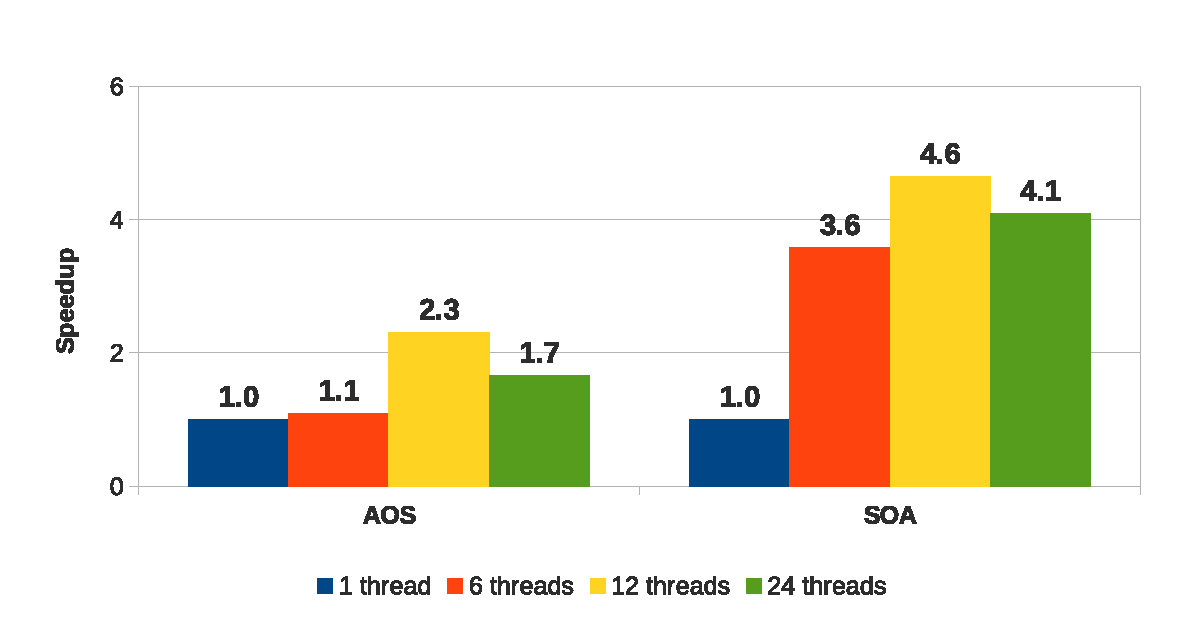
\includegraphics[width=\textwidth]{graph_comparison_omp.eps}
	\end{figure}
\end{frame}

\begin{frame}
	\frametitle{Limitations}
	\begin{itemize}
		\vfill
		\item Locality issues:
		\vfill
		\begin{itemize}
			\item Softened with SOA;
			\vfill
			\item Depends on the mesh structure;
			\begin{itemize}
				\item \texttt{gmsh} does not optimize the mesh;
			\end{itemize}
			\vfill
			\item Highly researched topic:
			\begin{itemize}
				\item Hoppe, 1999;
				\item Complex approach;
			\end{itemize}
			\vfill
			\item Specialized libraries:
			\begin{itemize}
				\item \texttt{parmetis};
				\item Unknown complexity;
			\end{itemize}
		\end{itemize}
	\end{itemize}
\end{frame}
\section{Distributed Memory}

\frame{\frametitle{Index}\tableofcontents[currentsection]}

\subsection{Partitioning}

\begin{frame}
	\frametitle{Distributed Memory: Mesh Partitioning}

	Mesh needs to be split between each processing unit.
	\begin{block}{Ideal partitioning method:}
		\begin{enumerate}
			\item Divide the mesh into $P$ partitions;
			\item Achieve good balance between partition sizes;
			\item Keep neighbourhood information;
			\item Minimize border between them, without compromising (2).
			\item Low partitioning overhead
		\end{enumerate}
	\end{block}

\end{frame}

\subsection{Implementation}

\begin{frame}
	\frametitle{Distributed Memory: Implementation}

	Division of the mesh based only on $x$ coordinate of cells:
	\begin{enumerate}
		\item Create ordered set of cells (key is $x$ coord)
		\item Sequentially assing $N/P$ cells to each process.
	\end{enumerate}

	\begin{multicols}{2}
		\begin{figure}
			\begin{center}
				\includegraphics[width=0.955\columnwidth]{foz_msh}
			\end{center}
		\end{figure}
		\pause
		\begin{figure}
			\begin{center}
				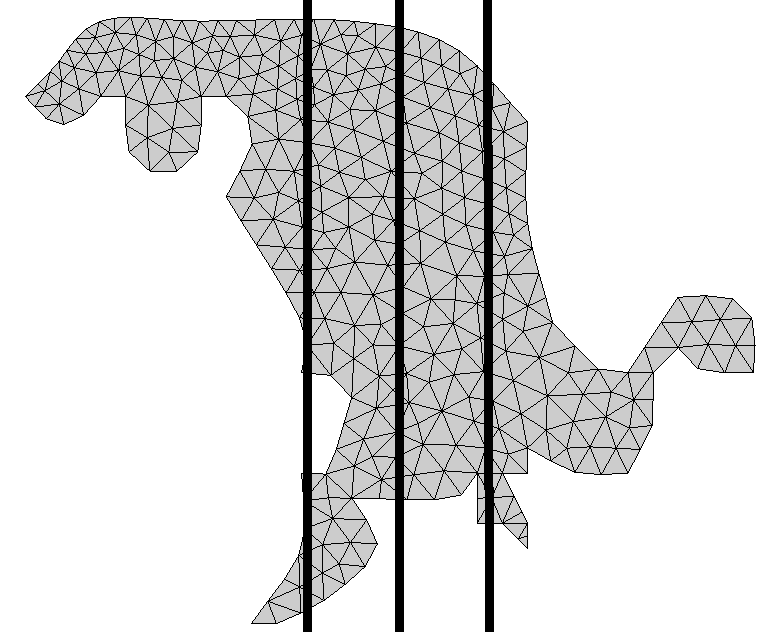
\includegraphics[width=0.955\columnwidth]{foz_p4_msh}
			\end{center}
		\end{figure}
	\end{multicols}
\end{frame}

\begin{frame}
	\frametitle{Distributed Memory: Implementation}

	\begin{block}{Two step communication}
		\begin{itemize}\itemsep=20pt
			\item Performed in two steps:
			\begin{enumerate}\itemsep=10pt
				\item Send to left / Receive from right
				\item Send to right / Receive from left
			\end{enumerate}

			\item Not homogeneous (no control over border size)

			\item Only 2 processes per node use the network
			\begin{itemize}
				\item Assuming best process asignement is used
			\end{itemize}
		\end{itemize}
	\end{block}
\end{frame}

\begin{frame}
\frametitle{Distributed Memory: Implementation}

	\begin{block}{Advantages}
		\begin{enumerate}\itemsep=10pt
			\item Simple concept and implementation
			\item Each partition has a left and a right neighbour
			\begin{itemize}
				\item[-] Communication in two steps only
			\end{itemize}
		\end{enumerate}
	\end{block}

	\begin{block}{Disadvantages}
		\begin{enumerate}\itemsep=10pt
			\item No control over size of border between partitions (communication)
			\item Sequential sort and distribution are slow
		\end{enumerate}
	\end{block}

\end{frame}



\section{GPU}

\frame{\frametitle{Index}\tableofcontents[currentsection]}

%
% IMPLEMENTATION
%
\frame{\frametitle{GPU}

	\begin{block}{Implementation}
		\begin{itemize}\itemsep=20pt
			\item \textit{Struct-of-Arrays}
			\pause

			\item \texttt{compute\_flux} and \texttt{update} directly converted to CUDA Kernels
			\begin{itemize}
				\item[-] Each iteration mapped to one CUDA Thread
			\end{itemize}
			\pause

			\item One aditional \texttt{reduction} kernel (later removed)
			\pause

			\item Data transfers only happen before the main loop
			\pause
			\begin{itemize}
				\item[] (exception: animation output, which is removed)
			\end{itemize}
		\end{itemize}
	\end{block}
}

\frame{\frametitle{GPU}
	\begin{block}{Load Balance}
		\begin{itemize}\itemsep=20pt
			\item workload of both kernels is homogeneous
			\pause
			\begin{itemize}
				\item[] (exception: for \update kernel, if number of edges per cell differs)
			\end{itemize}
			\pause


			\item Memory accesses are the main issue
			\pause
			\begin{itemize}
				\item[-] \computeflux will not access cells in order
				\item[-] Same problem for \update when accessing edges
			\end{itemize}

		\end{itemize}
	\end{block}
}


% \section{Experiment}

\frame{\frametitle{Index}\tableofcontents[currentsection,subsectionstyle=show/show/shaded]}

\begin{frame}
	\frametitle{Setup \& Methodology}

	\begin{block}{SeARCH Group Hex}
		\begin{description}
			\item [2] processors per node;
			\item [6] cores per processor;
			\item [-] Intel\textsuperscript{\textregistered} HyperThreading Technology;
			\item [2.66] GHz clock frequency;
			\item [12 to 48] GB of RAM;
		\end{description}
	\end{block}

	\begin{block}{Methodology}
		\begin{itemize}
			\item Limited execution: 5000 iterations;
			\item Median of 10 execution;
			\item 62 MB test case;
			\item Measurements focused on final speedups;
		\end{itemize}
	\end{block}
\end{frame}

\begin{frame}
	\frametitle{Speedups}
\end{frame}

% \input{slides/70-conclusion}

\begin{frame}[plain]
	\titlepage
	\begin{center}
		\Huge\bfseries - ? -
	\end{center}
\end{frame}

\end{document}%	end presentation
